\documentclass[a4paper,twocolumn,9pt]{jsarticle} %% A4で9ptで二段組にします
\usepackage[top=25truemm,bottom=25truemm,left=30truemm,right=30truemm]{geometry}
\usepackage[dvipdfmx]{graphicx} %% 画像挿入のパッケージ

%% タイトル
\title{タイトル}

%% 著者名
\author{名前}

%% 日付
\date{日付} %% \todayで今日の日付に

%% 開始
\begin{document}

%% 表紙
\maketitle

%% 内容ごとにセクションを分ける
\section{はじめに}
研究背景とか

\section{次に}
どういう研究なのかとか

%% サブセクションでさらに分けれる
\section{そのまた次に}
速度を$v$[m/s], 距離$l$[m]とすると, 以下の式で時間$t$[s]が求められる. \\
\[
s =\frac{l}{v}
\]
~~上の式より0$\sim$10000分かかると予想される. \\
\subsection{その1}
1つ目

\subsection{その2}
2つ目

\section{さらにその次}
図\ref{fig1}のテスト
%% \ref{ラベル名}で図番号を参照できる

%% 図を入れる
\begin{figure}[htbp]
 \begin{center}
  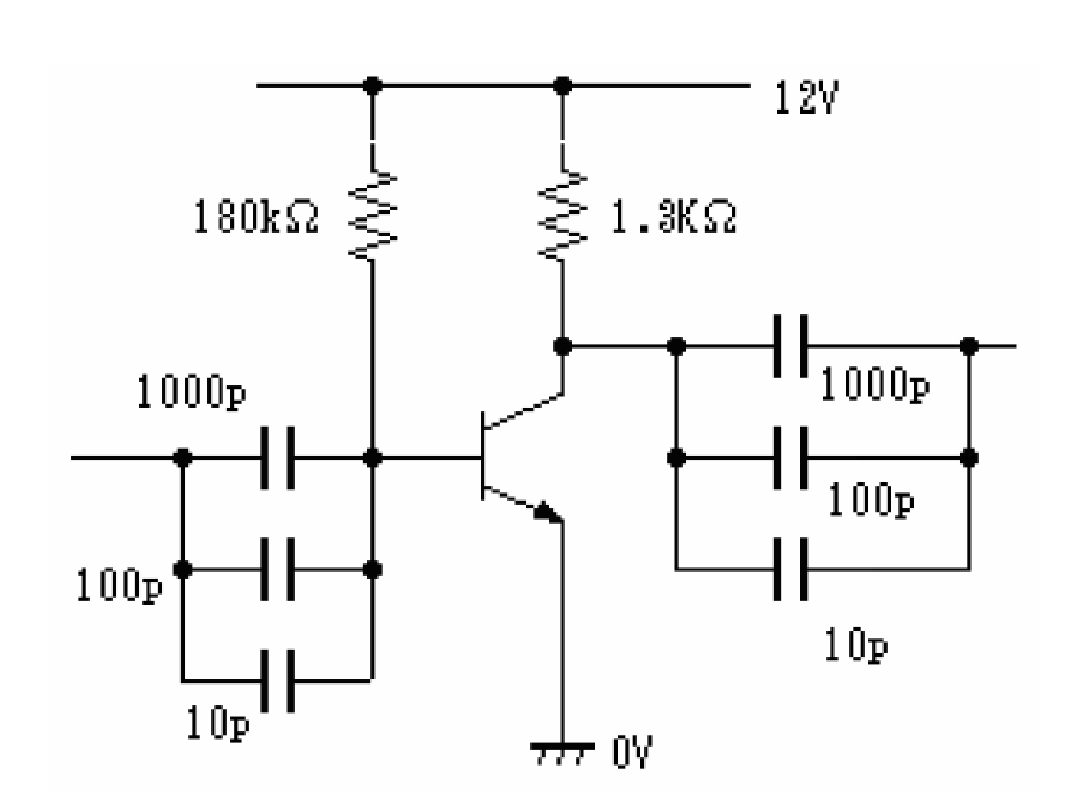
\includegraphics[clip,width=50mm]{fig.eps} %% includegraphics[scale=0.5]{~ で拡大縮小
   \caption{図題}
   \label{fig1}
 \end{center}
\end{figure}

%% 表を入れる
\begin{table}[hbtp]
  \caption{なんかの表}
  \label{sample_table}
  \centering
  \begin{tabular}{c|cc|cc}
\hline
    & \multicolumn{2}{c}{A} & \multicolumn{2}{|c}{B} \\
    & ch1 & ch2 & ch1 & ch2 \\
\hline \hline
値段 & 900 & 1130 & 3000 & 3100 \\
サンプル数 & \multicolumn{2}{c}{1} & \multicolumn{2}{|c}{11676} \\
\hline
  \end{tabular}
\end{table}

\section{おわりに}
できたこととか今度について

%% \cite{名前}で文献を参照できる
%% 参考文献を載せる
\begin{thebibliography}{9}
 \bibitem{bunken1} 文献1
 \bibitem{bunken2} 文献2
 \bibitem{bunken3} 文献3
 \bibitem{treatise} member1, member2, member3 : treatise. organization, issue, startpage-endpage, 2016
 \bibitem{book} name : title. orgnization, place, 2007
\end{thebibliography}

\end{document}
